% solar_prod.tex

\documentclass[12pt]{article}
\usepackage{setspace}
\usepackage[margin=1in]{geometry}
\usepackage{mathtools}
\usepackage{natbib} %for citet and citep
\usepackage{syntonly}
\usepackage{esdiff} %for writing partial derivatives
\usepackage{url} %for inserting urls
\usepackage{placeins}
\usepackage{textcomp}
\usepackage{amsmath}
\usepackage{graphicx}
\usepackage{booktabs}

\doublespacing % from package setspacs

\title{Are Solar Panels Commodities? Evidence of Quality Differences and Asymmetric Information from California}

\date{\today}

\author{Johannes Mauritzen \\ BI Norwegian Business School \\ johannes.mauritzen@bi.no\\\url{http://jmaurit.github.io}}

\begin{document}
 \begin{spacing}{1} %sets spacing to single for title page
	\maketitle

\begin{abstract}
 Solar panels should not be considered commodities. Considerable quality differences, as measured by degradation of production over time, are found between manufacturers. This has implications for pricing and competition in the market for solar panel systems. I test two implications from the the theory of asymmetric information of quality and find: 1.) Solar systems with third party owners display higher quality than those owned directly. 2.) Prices of solar panels are less correlated to quality for solar panels that are owned directly. I use multilevel models estimated by both maximum likelihood and Bayesian Markov Chain Monte-Carlo.
\end{abstract}

% \thanks{*I would like to thank...}
% JEL Codes: Q4, L71
 \end{spacing}

\section{Introduction}

Solar panels have been referred to colloquially in the power industry as being commodities. This is in reference to the high degree of competition, especially from Chinese manufacturers, that has dramatically driven down prices of solar panels in the last decade. This has made solar power price competitive without subsidies in many sunny locations. But it has also meant upheaval in the panel manufacturing industry with cheaper Chinese produced panels replacing panels produced in Europe, North America and Japan. Most recently, this led to the imposition of trade tariffs on Chinese produced solar panels by the US government.

However, a more thorough definition of a commodity generally includes a certain degree of fungibility. That is, the good from a certain producer will be largely interchangeable with the good of another producer. Brent crude oil produced by Statoil from the Norwegian North Sea and that produced by BP from the UK North Sea is sold at the same price, as established by an exchange. In a similar manner, the electricity produced by a solar panel at a certain location and time can also be considered a commodity.

However, an important differentiating characteristic between solar panels is the quality of these solar panels. This can be measured as both the failure rate of these panels as well as the degree of degradation of the panels over time. This can imply that certain manufacturers with superior quality could extract a premium in the market.

The combination of quality differences between panel manufacturers and the distributed nature of solar panel generation also opens up the issue of asymmetric information in the market for solar panels.

In an earlier paper \citep{mauritzen_whats_2015} I show that the boom in rooftop solar panel investment in California coincided with an adoption of a leasing business model by contractors. With leased panels, homeowners and small businesses do not pay upfront or own the panels on their roof. Instead, the contractor or a third-party own the panels and either collect a fixed monthly payment from the owner or charge a fixed price per kilowatt-hour (kWh) of electricity produced.\footnote{Charging for energy produced is often referred to as a power purchase agreement (PPA), but I here refer to all arrangements where the home- or business-owner does not own the solar panel system as a lease.}

Leased panels could be attractive for homeowners and businesses for several reasons. Not having to invest anything upfront would be attractive to those that are cash constrained. Lack of ownership could also be attractive to those concerned about the practicalities of maintaining and operating a small power station.

In addition, I argue that an issue of information asymmetry of quality could exist in the purchase of rooftop solar panel systems, and that leasing could provide a mechanism for alleviating this asymmetry. Homeowners and small business owners can not generally be expected to have the expertise to judge the quality of panels on their own. This issue could have been extenuated by the introduction of Chinese panels from manufacturers that were nearly completely new to the US and European markets in the time-frame studied and had little to build a reputation on.

Generally, the market for rooftop solar panels can be expected to be particularly vulnerable to issues of asymmetric information on quality. Solar panels can be characterized as an ``experience'' good, where an investor needs to learn about the quality through use. In particular, poor quality panels will tend to show a higher degradation of output over time than high quality panels. Even then, solar panel owners may find it difficult to measure the degradation as it can happen gradually, over many years.

More so, solar panel systems are expected to last at least 20 years, thus for all practical purposes, their purchase can be considered a one-shot investment. This eliminates repeat buying as a mechanism for ensuring quality. In the literature, warranties are often suggested as a strong signal of quality. However, warranties may be a relatively weak assurance of quality in the market for solar panels as both contractors and manufacturers are relatively new, tend to be heavily indebted and some have recently shown a tendency to go bankrupt.

Given the difficulty of judging quality and lack of market mechanisms to signal quality, the established economic theory on the subject would suggest that the market may tend to provide low-quality panels \citet{tirole_theory_1988}.

However, over the period from 2010 to 2014, many of the larger solar contractors moved to leasing solar power systems to homeowners. The introduction of a leasing model could potentially get over this information asymmetry problem by shifting ownership to the large contractors that install and finance the solar systems. These contractors can then in turn take steps such as testing panels and visiting manufacturing sites to ensure quality of suppliers.

A testable implication that emerges is then that the quality of panels - as measured by degradation of output over time - is better in systems that are leased.  In this paper, I use a data set of California solar power systems that includes monthly production data. I measure the average degradation of production over time as a proxy for the inherent quality of solar panel system.

Testing for the degradation in production of more than 3000 panels is however problematic using traditional econometric models based on frequentist approaches. The production patterns of the solar panels could be expected to vary greatly depending on location, equipment, size as well as other factors. The inclusion of many fixed effects to control for these factors would likely lead to over-fitting. That is, the model may have a good fit to the data, but will tend to have poor out-of-sample predictive power \citep{gelman_bayesian_2013}.

As a solution, I use a Bayesian hierarchical model estimated using Markov Chain Monte Carlo (MCMC) simulation techniques. The main benefit of using a Bayesian multilevel model is that we can fit a complex model with many hundreds of parameters, while avoiding problems of over-fitting and issues of multiple comparison in inference by relying on partial pooling of the parameters. The main finding is that solar panel systems that were leased tend to show significantly less degradation over time than those that were sold outright.

The issue of how information asymmetries of quality affects market outcomes, first introduced by \citet{akerlof_market_1970} is one of the main topics in the modern industrial organisation literature. Ch. 2 of \citet{tirole_theory_1988} and accompanying citation list provides a good overview of the theoretical foundations of this topic.

Early theoretical work of particular relevance to this paper includes \citet{chan_prices_1982}, whom model the situation where information on quality is costly rather than directly unavailable and where quality is endogenous to the seller - in other words the seller can choose the level of quality of its product. Under these assumptions, the authors predict several equilibrium - essentially markets for both high and low quality products depending on the extent to which the buyer is informed.

Reputation - or lack thereof - plays a particularly important role in this market. Most of both the solar installers and panel manufacturers are relatively new firms - especially the increasingly dominant Chinese solar panel producers,  \citet{shapiro_consumer_1982} explores the role of reputation, and finds that because reputation is effective only with a lag, the "steady-state" quality level chosen by a seller should be lower than in the scenario with perfect information.

Expanding empirical literatures also exist on asymmetric information of quality - especially in the marketing, finance and accounting fields. In accounting, the issue of firm quality and voluntary disclosure in regulatory filings as a signal has received broad attention by empirical researchers. \citet{healy_information_2001} review the early literature. Empirical studies in finance have, for example, looked at issues of adverse-selection in Initial Public Offerings \citep{michaely_pricing_1994} and small business lending \citep{petersen_benefits_1994} among many other topics.

The literature in the marketing field may be more relevant to this paper, as it is particularly concerned with the effects of information asymmetry on purchases of consumer durables. The effects of signaling on quality - usually in the form of advertising - is particularly important in the field. \citet{kirmani_no_2000} provide an overview of this literature.

The use of leasing, discussed in this article, can be seen as a form of costly signaling about quality, however leasing plays more than just an informational role since it also transfers much of the risk of poor quality to the contractor.

Traditionally, energy generation has been an activity undertaken by large, specialized firms with specialized knowledge and resources. The role of information asymmetry in investment and purchase decisions has likely been seen as a secondary issue, and to my knowledge, no literature exists on the role of such informational issues in the industry.

However, the growth of distributed energy technologies, like solar panels, has added new focus on behavioral and information issues related to energy investments by homeowners and small businesses. In turn, a growing literature is forming around solar power investment behavior of homeowners and small businesses.

For example \citet{dastrup_understanding_2012} argue that solar panels can not be considered a pure investment good, but are also bundled as a type of green conspicuous consumption - showing evidence for a ``solar price premium'' in homes with solar panels. \citet{bollinger_peer_2012} study the the role of peer effects in solar power adoption. They find evidence that the adoption of solar panels by homeowners in a certain zip-code will increase the probability that other households in that zip-code will install solar panels.

Despite the growth of the literature on investments in distributed energy, to my knowledge this is the first paper to identify and directly test implications of information asymmetry in the expanding industry. The paper has implications for regulation and subsidy policy for the expanding distributed energy industry.

\section{California Solar Initiative, Data}

The data used in this paper is an intersection of two datasets from the California Solar Initiative (CSI). The California Solar Initiative is a state-wide program that gives incentives for installing grid-connected solar panels systems. The incentives are based on performance. For smaller systems, typical of most residential and small business installations, this incentive was given in the form of an upfront payout based on the capacity and the expected performance of the system.

Larger systems were required to accept a performance based incentive based on actual production over 5 years (60 months). From the beginning of the program in 2007 this was defined as those over 100kW, but was lowered to 50kW from January 2008 and 30kW from January 2010. Solar panel installations of all sizes have the option of getting an incentive based on actual performance.

CSI provides data on all grid-connected solar panel systems installed in California since January 2007. In addition, CSI provides another data set of monthly production data from the solar panel systems that received production incentives. The data is openly available on the website of CSI. \footnote{\url{http://www.californiasolarstatistics.ca.gov/current_data_files/}}. A cleaned and merged data set that I use in the following analysis can be found on my website at \url{jmaurit.github.io#buy_or_lease}.

Below are the key variables present in the CSI installation data:

\begin{itemize}
\item Installation date
\item Location: address, zip code, county
\item System capacity
\item Name of system owner, host, and contractor
\item Panel and inverter manufacturer
\item Third party owner (leased)
\item Use of single or double axis trackers
\item Year of installation
\end{itemize}

The installation data can be matched with the production data for those installations receiving a production subsidy. I include only those installations that have been producing for at least 3 years (36 monthly observations), where the maximum number of observations in this data is 5 years (60 months) of production data.

I removed systems from the dataset that may have had reporting errors. for example I removed systems where production was reported to be higher than what would be theoretically possible from a solar power system with a given nameplate capacity. I also removed systems that reported 0 production in a period. This could also be an indication of quality if zero production indicates a malfunction in the system. However it is not possible to identify which zero observations reflect malfunctions versus reporting issues or other non-quality issues.

Figure \ref{tot_production} shows the production for the included solar panel systems over time. The seasonality of the systems over the calendar year is clear, and needs to be accounted for in the statistical analysis.

\begin{figure}
	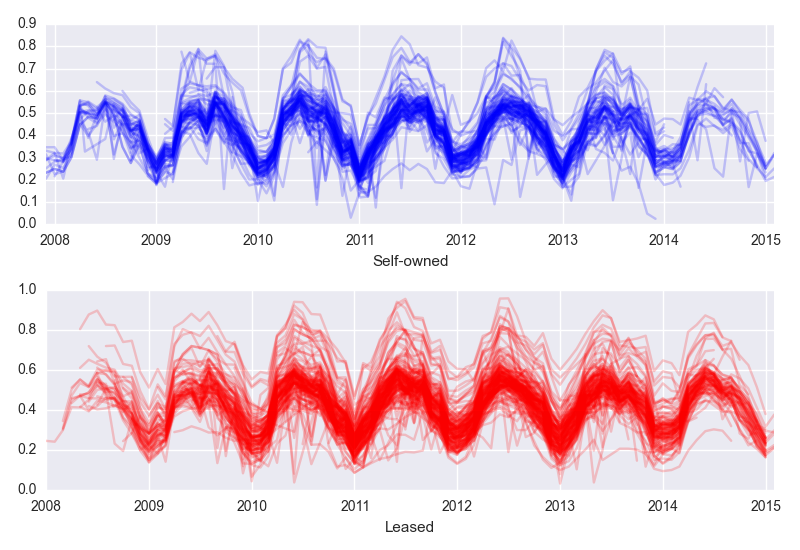
\includegraphics[width=1\textwidth]{tot_production.png}
	\caption{Production over time from California solar panels, Host owned and leased. Production index reflects monthly production in kWh normalized by capacity multiplied by 30.5*12 to reflect a rough estimate of maximum day-light hours in a month.}
	\label{tot_production}
\end{figure}

The main methodological goal of this paper is to make an unbiased estimate of the slope of the average degradation of solar panels - comparing the slopes between groups of systems that are leased and bought outright. These estimates should also control for seasonality and idiosyncratic factors between solar power systems.
A simple example of fitting a straight lines through two production series is shown in figure \ref{example_prod} - here as a simple single variable OLS estimate.

\begin{figure}
	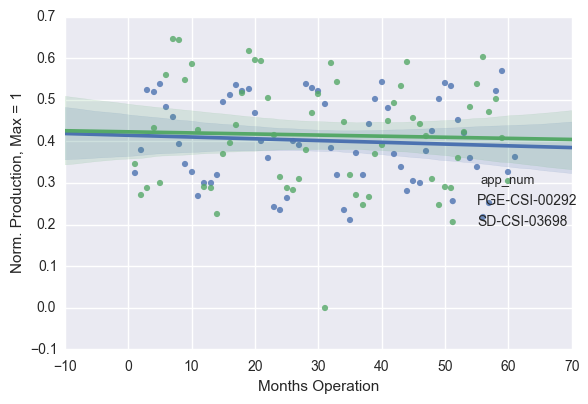
\includegraphics[width=1\textwidth]{example_prod.png}
	\caption{The main methodological task in this paper is to make an unbiased estimate of the slope of the average degradation of production over time. The figure demonstrates a straight line fitted to a time series from a single solar power system.}
	\label{example_prod}
\end{figure}

The question of interest and the structure of the available data suggests a hierarchical structure to the empirical model. The individual production data are grouped by the different solar panel systems. Each system is then in turn grouped into categories of leased or host-owned. As mentioned, seasonality must also be adequately accounted for as well as other factors such as geographic location, use of tracking and idiosyncratic variation from one solar panel system to another.

\section{Linear Mixed Effects Models Estimated by Maximum Likelihood}

\subsection{Testing for differences between module manufacturer}
Following the notation of \citet{bates_fitting_2015}, the conditional distribution of the response variables, $y$ in a multilevel model can be written compactly as in equation \ref{equation:lme_simple}. Here $\mathbf{\beta}$ is a p-dimensional coefficient vector (or "fixed effects") of the $n times p$ matrix of (p-1) explanatory variables $\mathbf{X}$ plus intercept term. $\mathbf{Z}$ is an $n \times q$ model matrix of the variables whose groups are to be modelled directly with corresponding vector of coefficients, or "random effects" $\mathbf{B}$ that are fixed at values $\mathbf{b}$.\footnote{The use of "random" refers to the fact that these groups are assumed to be specific to the sample. Many applications of mixed effects model thus treat the varying group coefficients as group-level error-terms, thus the "random" label. Still, interpreting coefficients as group varying or as group error terms is mathematically equivalent.} Here $q$ is a dependent on the number of terms, $k$, that are allowed to vary by group and the number of groups, $l$ for each term: $q=\sum_i^k q_i = \sum_i^k l_i p_i$.  $\mathbf{W}$ is a diagonal matrix of known prior weights. $B$ is distributed as multivariable normal with zero mean and where $\Sigma$ is variance-covariance matrix.

\begin{align}
(y|\mathbf{B=b} &\sim \mathcal{N}(\mathbf{X\beta + Zb}, \sigma^2\mathbf{W^{-1}}))\\
B &\sim \mathcal{N}(\mathbf{0,\Sigma})
\label{equation:lme_simple}
\end{align}

Models of this form can be solved efficiently using a penalized maximum likelihood routine. For further details of both the model and routine, I refer to \citet{bates_fitting_2015}.

To test whether I can detect quality differences between module manufacturers, I need to first estimate a restricted comparison model. I write the restricted comparison model explicitly in equations \ref{eqn:observation_level_rest} and \ref{eqn:system_level_rest}.

In this model, the transformed production variable, $prod\_scaled_{i}$ for observation $i$ is distributed normally with the mean modelled as a linear function of an intercept term $a_s$, a slope term, $b_s$ on the transformed months of operation variable $months\_operation\_scaled$, and a set of dummy variables representing the month of year, $\mathbf{month}$. Notice that the intercept and slope are indexed by $s$, indicating that they are allowed to vary by the individual system. Thus in this model formulation I take into account the groupings by system, explicitly modelling varying relative initial production values (intercepts) and degradation over time (slope). Moving up a level, the estimated $a$ and $b$ parameters are in turn modelled as multivariate normal.

\begin{align}
prod\_scaled_{i} &\sim N(\mathbf{month} + a_s + b_s months\_operation\_scaled_{i}, \sigma^2)\\
\label{eqn:observation_level_rest}
\begin{pmatrix}
  a\\
  b
\end{pmatrix}
&\sim N
\begin{pmatrix}
  \mu_a\\
  \mu_b
\end{pmatrix},
\begin{pmatrix}
  \sigma_a^2 & \rho \sigma_a \sigma_b \\
  \rho \sigma_a \sigma_b & \sigma_b^2
\end{pmatrix}
\label{eqn:system_level_rest}
\end{align}

The inclusion of the matrix of month dummies $\mathbf{month}$ controls for seasonal variation across all systems. This is a simplified way to model seasonality, but because the data is itself at a monthly frequency, and the seasonality is not of direct importance, this should suffice. As long as un-modeled variation in seasonality is not correlated with the long-run slope of production, the point estimates for the slope should be unbiased.

To test whether quality varies among module manufacturers, I simply add panel manufacturer as an extra hierarchy to the model. In this model, the observation level regression is identical to the restricted comparison model as in equation \ref{eqn:observation_level_rest}. The system-level intercepts, $a$, and slope, $b$, terms are also modelled as a multivariate normal. But the mean values of the multivariate normal distribution, $mu_a$ and $mu_b$, are now indexed by $m$, representing that they are allowed to vary by module manufacturer.
\begin{align}
\begin{pmatrix}
  a\\
  b
\end{pmatrix}
&\sim N
\begin{pmatrix}
  \mu_{a[m]}\\
  \mu_{b[m]}
\end{pmatrix},
\begin{pmatrix}
  \sigma_{a[m]}^2 & \rho \sigma_{a[m]} \sigma_{b[m]} \\
  \rho \sigma_a \sigma_b & \sigma_b^2
\end{pmatrix} \\
\mu_{a} &\sim N(\theta_a, \sigma_{mu_a}^2) \\
\mu_{b} & \sim N(\theta_b), \sigma_{mu_b}^2)
\end{align}

If there is no significant variation between the module manufacturer groupings, this model collapses into the restricted comparison model, which is the null hypothosis. Figure \ref{sfig:sys_slope_fig} gives a visual summary of the system-level slope terms ordered from lowest to highest. The lines represent approximate 95\% confidence intervals around the point estimate. One anomaly we can notice is that a handful of the systems have slopes that are estimated to be positive. This is clearly problematic if we wish to interpret the slope coefficient as degradation over time. I address this in the full Bayesian model without resorting to excluding data.

\begin{figure}
\begin{minipage}{.48\textwidth}
  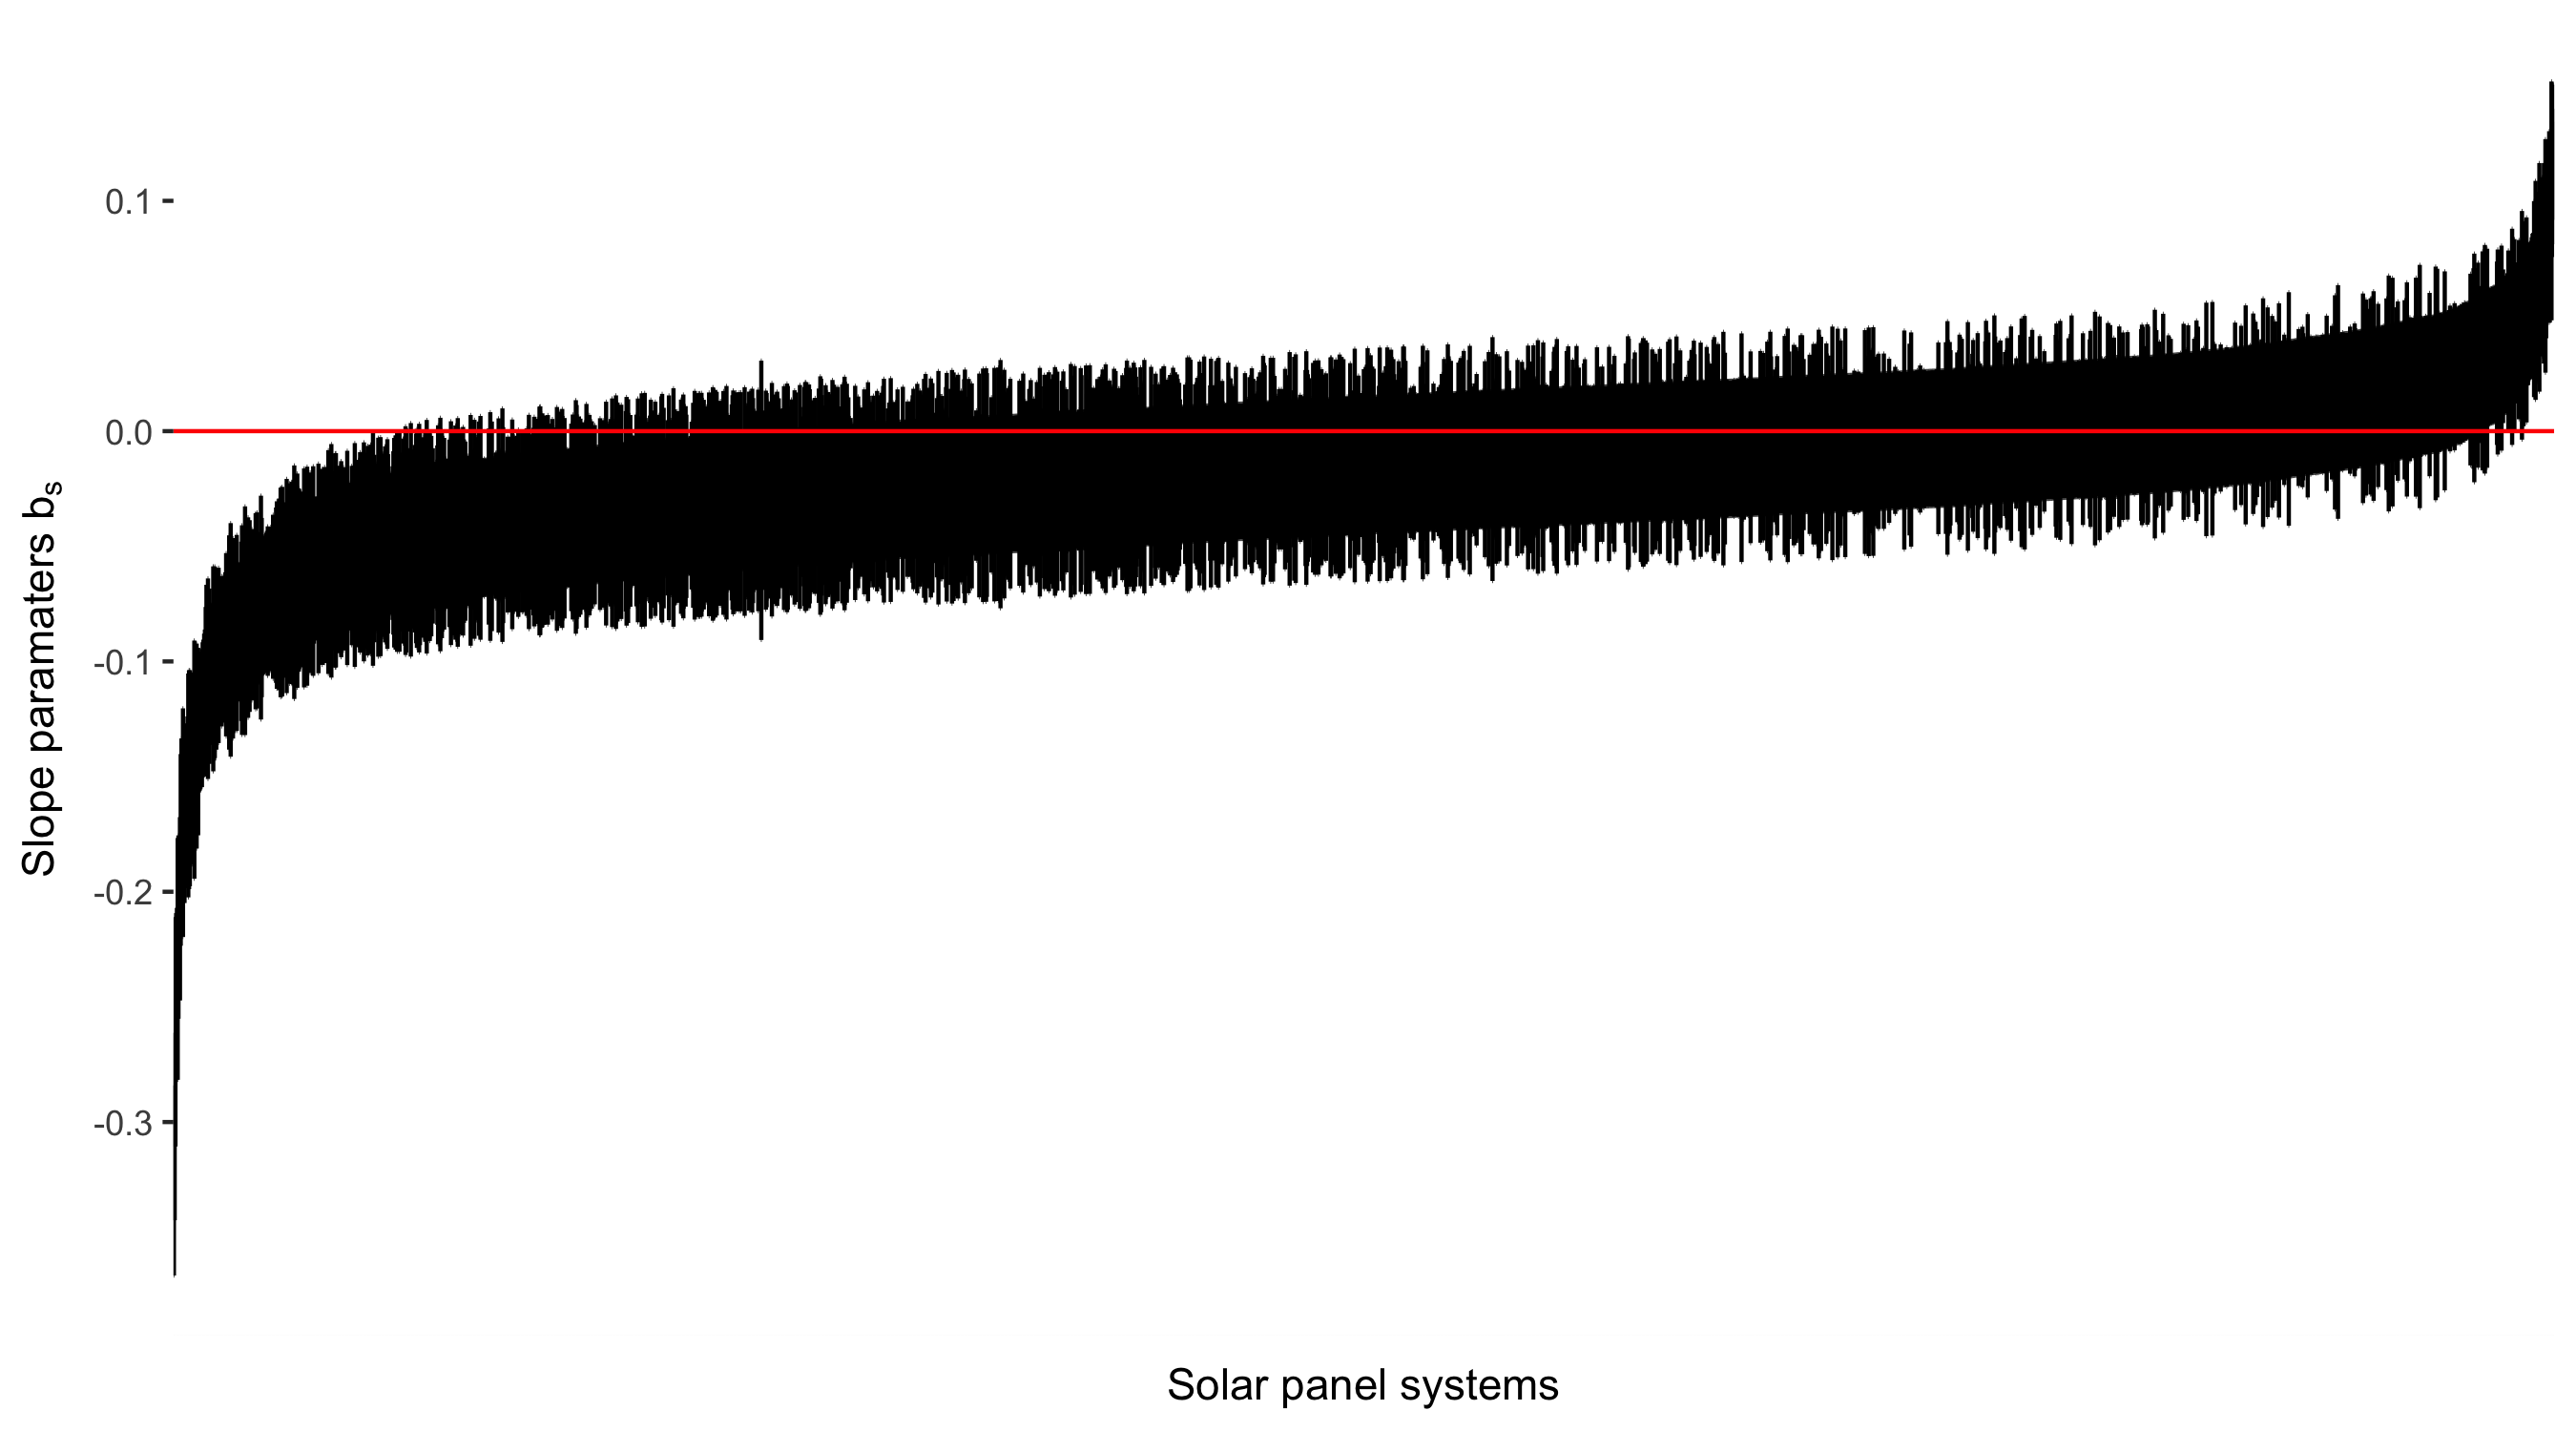
\includegraphics[width=1\linewidth]{figures/sys_slope_fig.png}
  \caption{Approximate 95\% confidence intervals around maximum likelihood point estimates of system-level slope terms, ordered from lowest to highest.}
  \label{sfig:sys_slope_fig}
\end{minipage}\hfill
\begin{minipage}{.48\textwidth}
  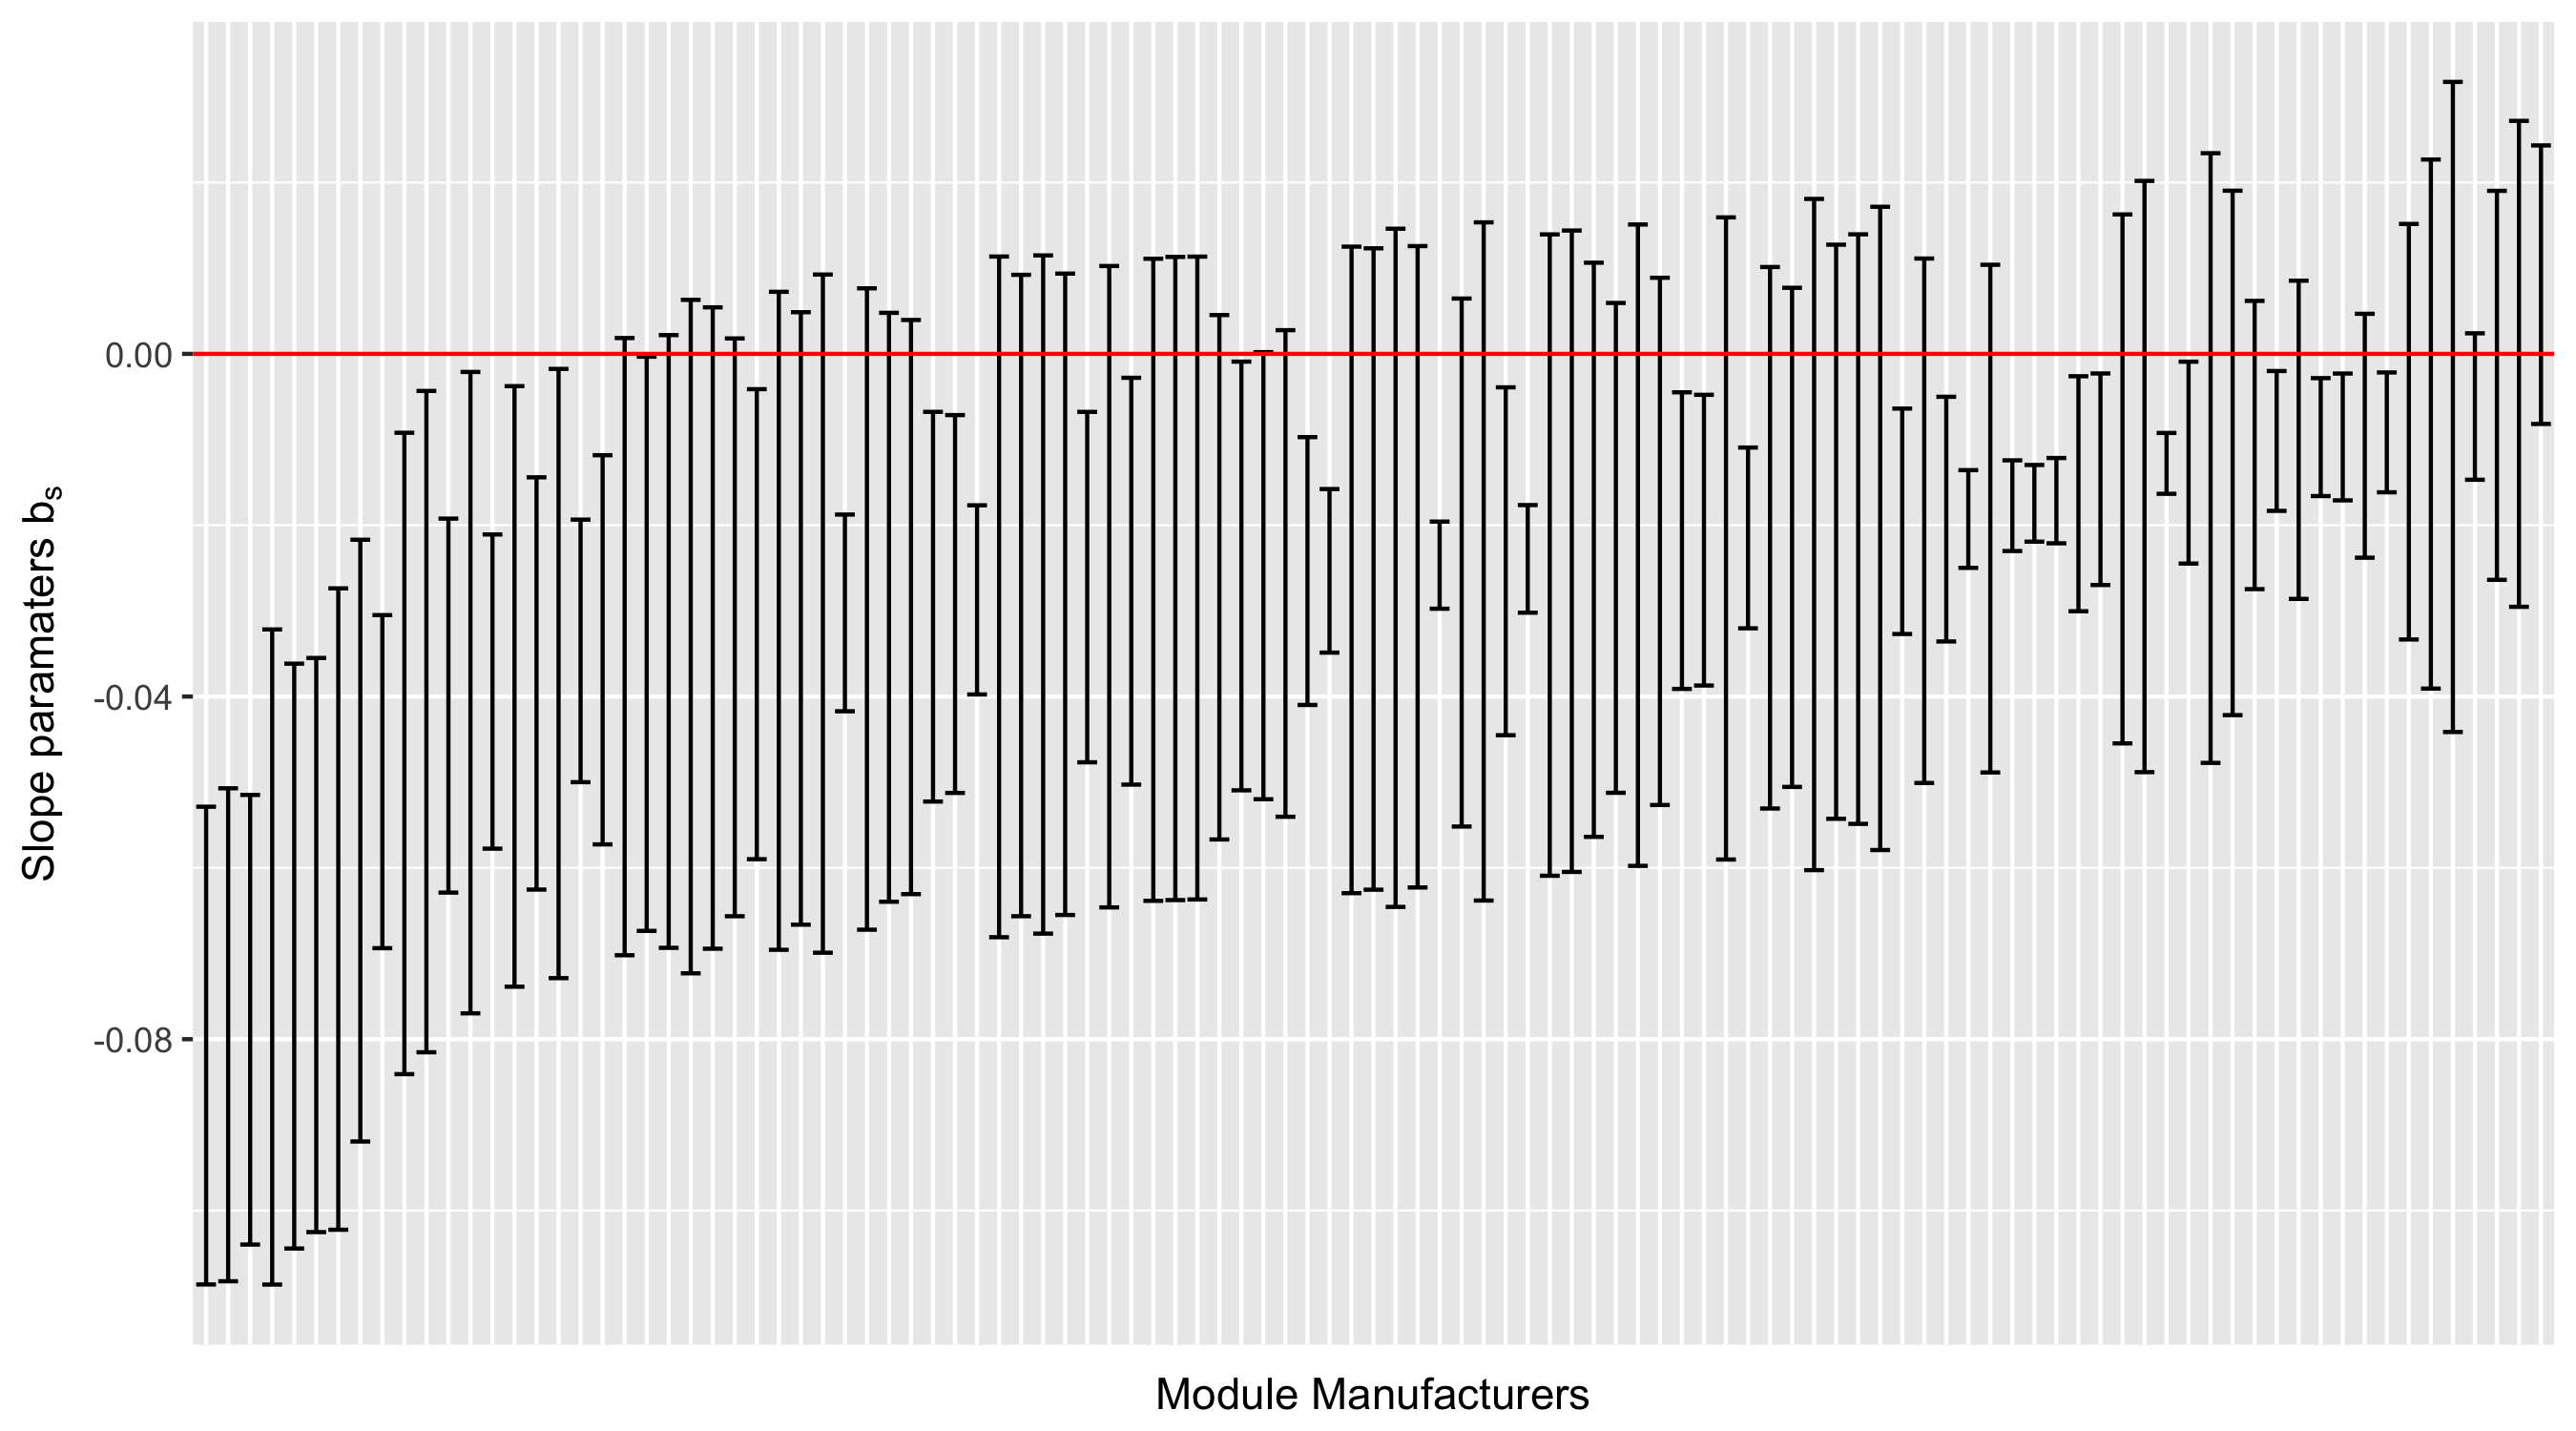
\includegraphics[width=1\linewidth]{figures/nested_manuf_fig_final.png}
  \caption{Approximate 95\% confidence intervals around maximum likelihood estimators of manufacturer-level slope terms $\mu_b$, ordered from lowest to highest.}
  \label{sfig:nested_manuf_fig}
\end{minipage}
\end{figure}

\ref{sfig:nested_manuf_fig} gives a summary of the estimated manufacturer-level mean slopes. Again the lines represent 95\% confidence intervals around the point estimates. Visually, we can see substantial variation in quality between the manufacturer groups. We can more formally test the hypothesis that manufacturer groupings improve the explanatory power of the model by comparing to the restricted model with an LM test. The results are shown in table \ref{tbl:lm_commodity}. The information criteria measures (AIC, BIC) are both lower, indicating a better predictive power of the model with manufacturer groupings. The chis-square statistic also indicates that the model with manufacturer groupings substantially improves model performance.

\begin{table}
  \begin{tabular}{rllllllll}
  \toprule
    Model &  DF &   AIC &   BIC &  logLik &  deviance &  Chisq &  Chi df &  Pr(>Chisq) \\
    \midrule
             Null &  17 &  8805 &  8976 &   -4385 &      8771 &     -- &      -- &          -- \\
    Grouped Manuf. &  20 &  8430 &  8631 &   -4195 &      8390 &    381 &       3 &     2.6e-82 \\
  \bottomrule
  \end{tabular}
  \label{tbl:lm_commodity}
\end{table}

The first result, of which the evidence appears to be quite strong is that solar panel systems do appear to vary substantially in quality between module manufacturers. Given that module quality is an important differentiating characteristic of panels, it is then difficult to formally define solar panels as commodities.

\subsection{testing for differences in quality between leased and host-owned solar power systems}

Provided the evidence that solar panel systems are not commodities and that substantial differences in quality do exist between manufacturers, we can now move on to the testable implication that comes from a combination of standard economic theory of asymmetric information and a descriptive understanding of the market that suggests the market for solar panels could plausibly be subject to issues of asymmetric information of quality.

From our informal model of asymmetric information where we see host owners of solar systems as being low-information types, while owners of leased panels as being high information types, we would predict that on average leased panels will display higher quality over time. To test this directly with the data, I only need to do a slight modification of the model in the previous subsection. Instead of grouping the system-level coefficients by manufacturer, I now group into whether the solar power system was leased or not, as indexed by $l$. We can then compare the average slopes between these groups. For convenience the model is presented in full in equations \ref{eqn:observation_level_rest2}.

\begin{align}
prod\_scaled_{i} &\sim N(\mathbf{month} + a_s + b_s months\_operation\_scaled_{i}, \sigma^2)\\
\label{eqn:observation_level_rest2}
\begin{pmatrix}
  a\\
  b
\end{pmatrix}
&\sim N
\begin{pmatrix}
  \mu_{a[l]}\\
  \mu_{b[l]}
\end{pmatrix},
\begin{pmatrix}
  \sigma_{a[l]}^2 & \rho \sigma_{a[l]} \sigma_{b[l]} \\
  \rho \sigma_a \sigma_b & \sigma_b^2
\end{pmatrix} \\
\mu_{a} &\sim N(\theta_a, \sigma_{mu_a}^2) \\
\mu_{b} & \sim N(\theta_b), \sigma_{mu_b}^2)
\label{eqn:lease_model}
\end{align}

A visual summary of the results are shown in figure \ref{lease_sys_fig}. Again, the vertical lines represent approximate 95\% confidence intervals over the point estimates for the system-level slope terms, $b_s$. But here the the slope estimates are grouped into host-owned (left) and leased (right). The estimated group means are shown as horizontal lines. At the scale of the figure, the effect appears small, but the average slopes are estimated to be significantly different from each other at the 95\% confidence interval. The difference is also economically significant. Extrapolating out from the difference in the point estimates between leased and host-owned suggests that on average a leased system can expect to be producing 11\% more power after 10 years compared to an otherwise identical solar panel systems.

\begin{figure}
	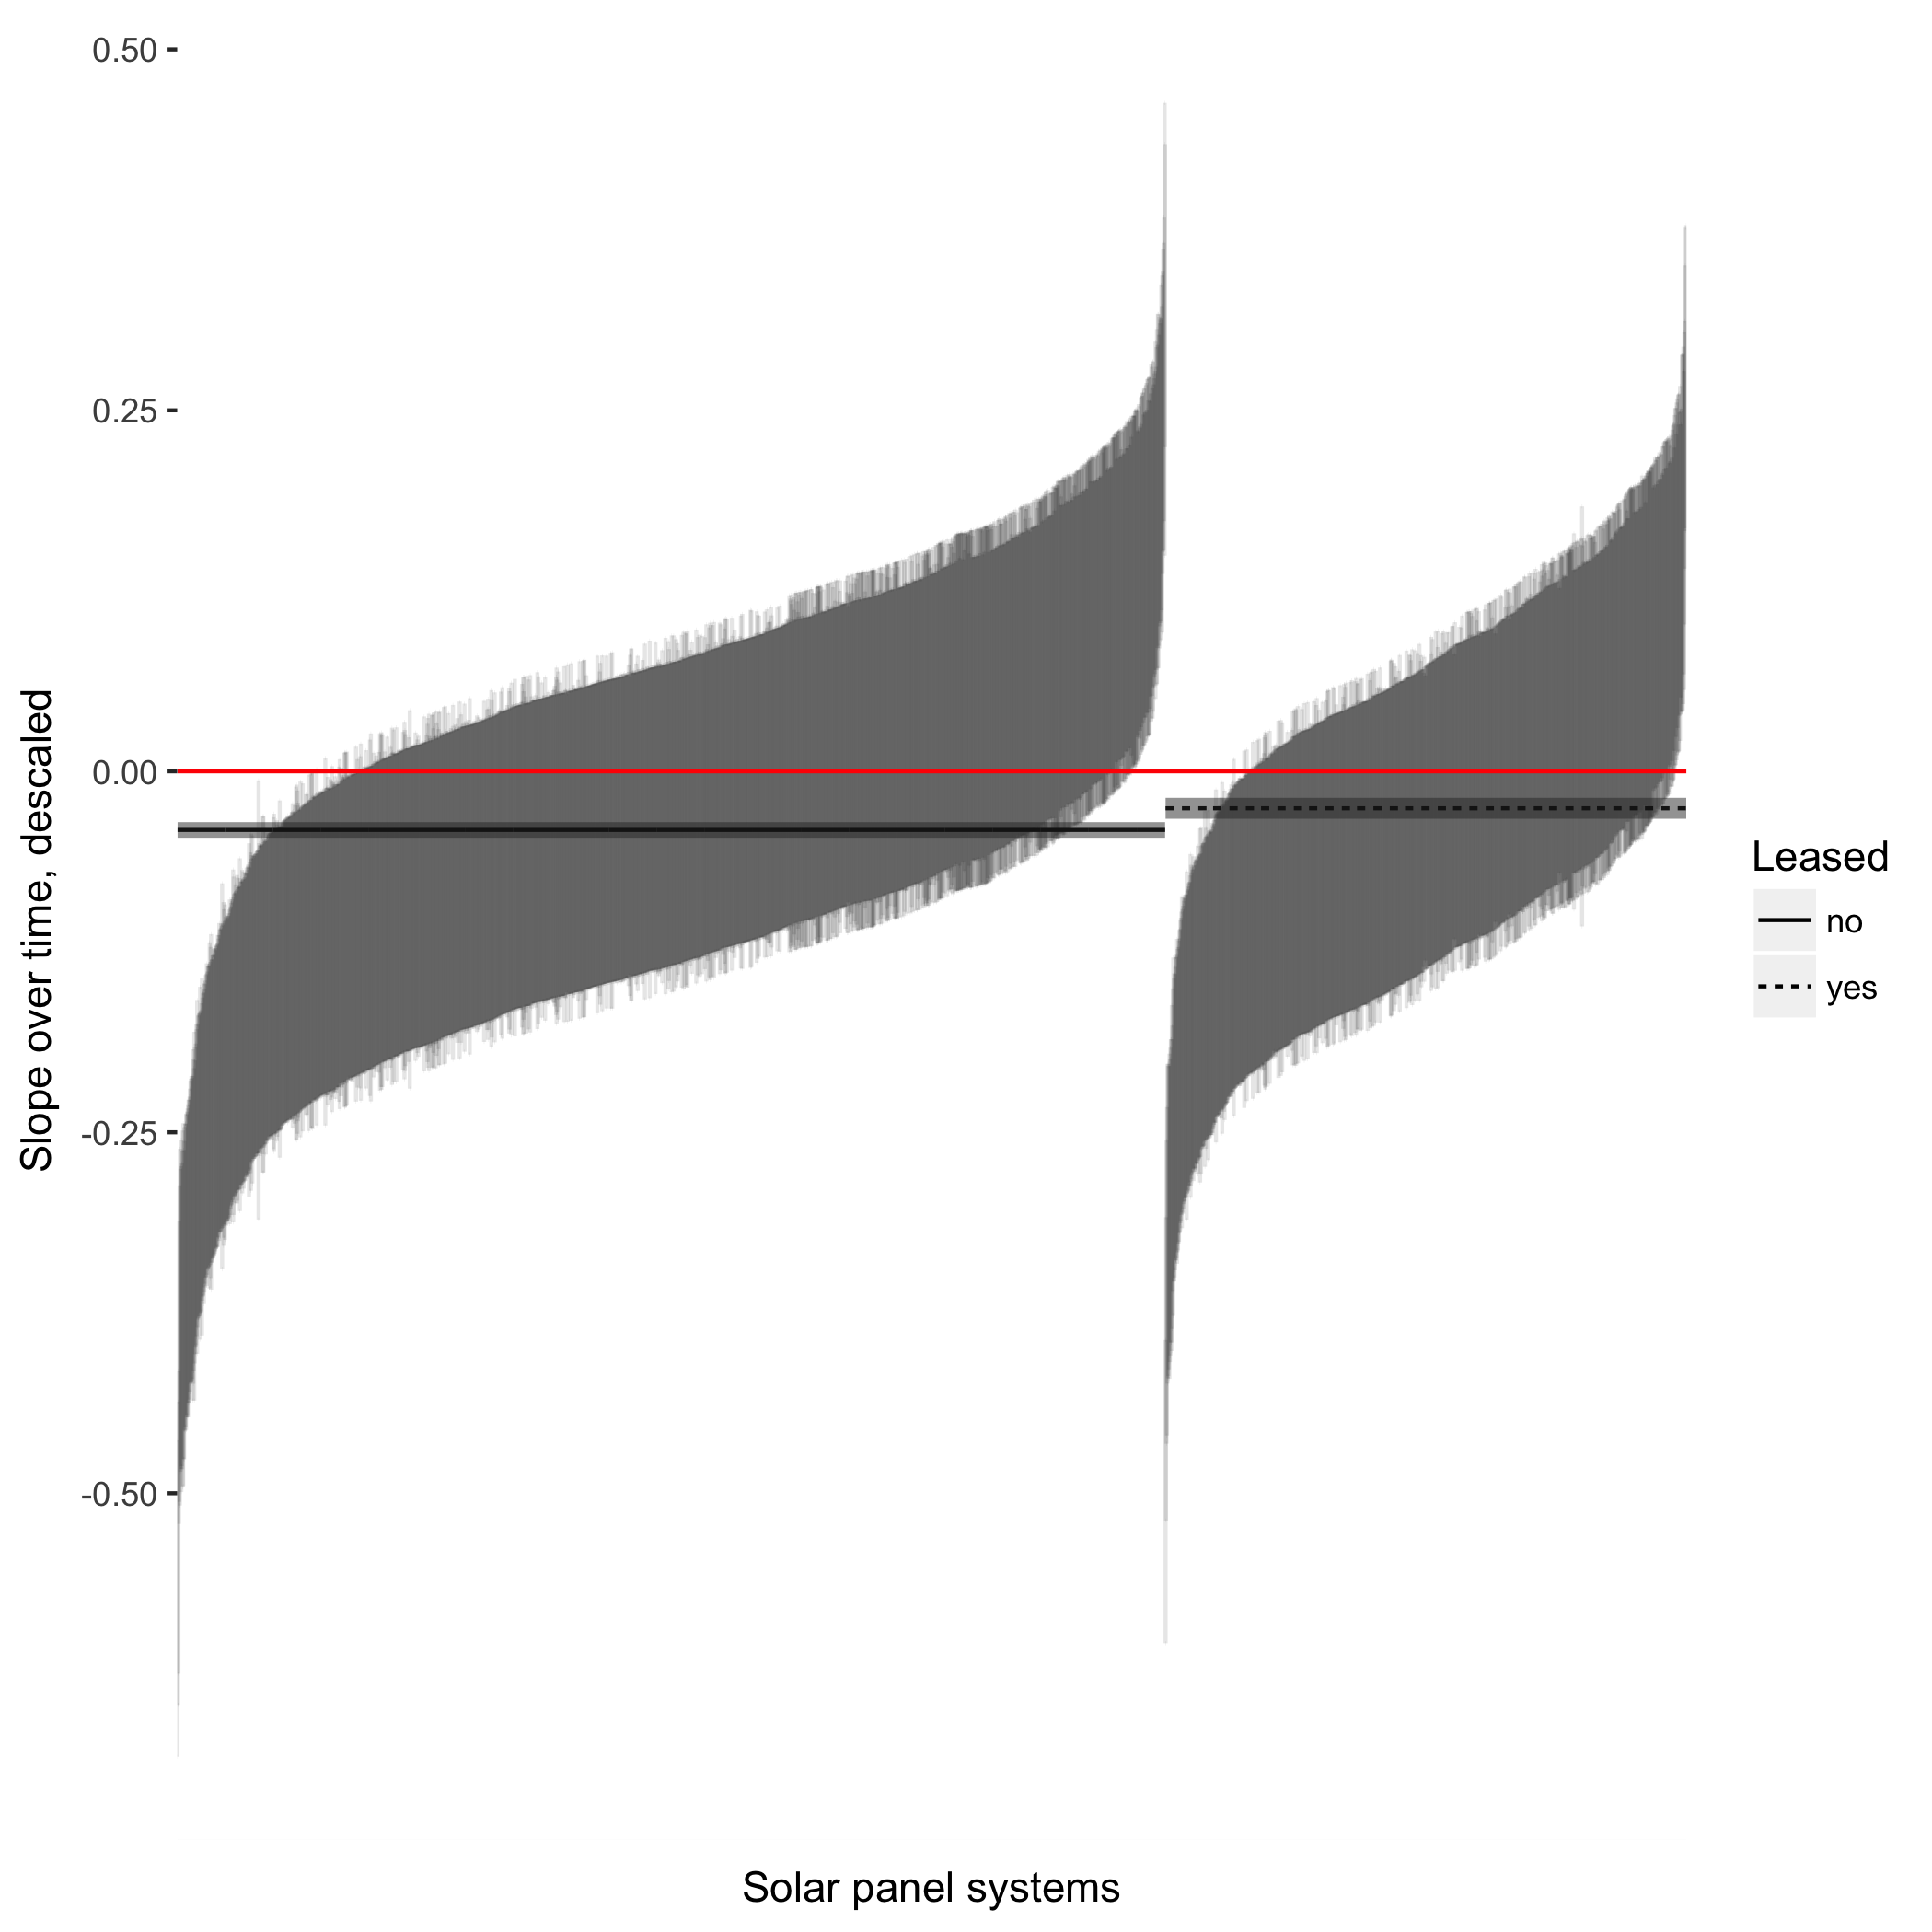
\includegraphics[width=.8\textwidth]{figures/lease_sys_fig.png}
	\caption{A visual summary of the estimation results. The vertical lines again represent the estimated system-level slope coefficients.}
	\label{lease_sys_fig}
\end{figure}



\section{Full Bayesian multilevel model estimated by Markov Chain Monte Carlo}

Until now, I have used relatively parsimonious models with few fixed-effects covariates and only one or maximum two hierarchies ("random effects").  Ideally, I would like to estimate a full probability model with all relevant and available covariates and hierarchies. First and foremost so that the parameters of interests to the testable implications can be estimated from one model. But also, citet{bar_random_2013} shows using monte-carlo simulations that mixed effects models that have the maximum random effects structure justified by the model and data, provide the best out-of-sample prediction. Estimating mixed effects model by maximum likelihood is efficient and straight-forward. However, convergence of the maximum likelihood routine is not guaranteed under richer models with more hierarchies and larger number of paramaters to be estimated.

Specific to my model, I wish to estimate a model where the variable for cost per-kw is included as an interaction that varies by system and module manufacturer. I also wish to have a model where both system, module manufacturer and leasing hierarchies are estimated simultaneously. I am not able to obtain convergence of the maximum likelihood routines under this rich model.

As a solution, I build a fully Bayesian multilevel model\footnote{I purposefully change my nommenklature here and refer to the Bayesian model as a "multilevel model" to distinquish it from the models estimated by maximum likelihood, which I refer to as a linear mixed effects model. This distinction is however mostly artificial. Both models resemble each other closely in structure. "Multilevel model" is however a broader term. There is no restriction to linearity, for example. Models with non-linear or non-parametric components can also be incorporated and estimated with MCMC.} estimated by Markov Chain Monte Carlo (MCMC) simulation techniques.

The main advantage to using the Bayesian techniques here are practical rather than philosophical. Models up to levels of nearly arbitrary richness can be estimated, with computation time and available data being the main constraints. Inference is also well defined and exact,\footnote as opposed to the approximate inference from maximum likelihood.

A Bayesian MCMC approach does also have some attractive properties. Results are presented estimates of marginal posterior distributions over coefficients of interest, which can be interpreted directly and intuitively as probabilities. Group-level variances are not constrained to be equal and assumptions of normality of the likelihood and posterior distributions can be loosened. Several excellent discussions of Bayesian techniques are available, see \citet{gelman_bayesian_2013}, \citet{kruschke_doing_2014}, or \citet{mc}

Figure \ref{solar_prod_bayes_diag} shows the structure of the model. Starting from the bottom, the individual production data are log transformed and modeled as having a Cauchy distribution with mean $y_hat$ and variance $sigma^2$. $sigma^2$ is in turn given a half-Cauchy prior.

The use of the Cauchy and half-Cauchy distribution reflects that a large in magnitude effect of around 5 or greater on the logit scale is highly unlikely in logistic regressions where all non-binary data has been transformed to have mean zero and standard deviation 1 - which I have done. In addition, the Cauchy distribution will give answers even under complete separation, and avoids computational problems inherent in assigning completely non-informative priors in multilevel models \citep{gelman_weakly_2008}.

Going up a level, $y_hat$ is modeled as having random group-level intercepts $\beta_{0,j}$, where j represents the j-th of $J$ solar panel system. The $\beta_{0,j}s$ are in turn modeled as function of system size, county, whether solar trackers are used, and a random effects term $re_j^0$.

In a similar manner the J $B_j$ coefficients are modeled as a function of whether the system is leased, $\mu_{lease}^1$, the host sector of the installation, the county, use of tracking, installation year and a random effects term $re^1_j$.  The question of interest - whether leased solar systems display a lower degree of degradation over time than those sold outright - can then be expressed as the distribution of the difference of the $mu_{lease}$ parameters: $\mu_{lease=1} - \mu_{lease=0}$.

Finally, to take into account the seasonality of the monthly data, random effects for each of the 12 months are estimated with a $Cauchy(0,4)$ prior on each parameter. The remaining hyper-parameters are given Cauchy or half-Cauchy priors.

\begin{figure}
	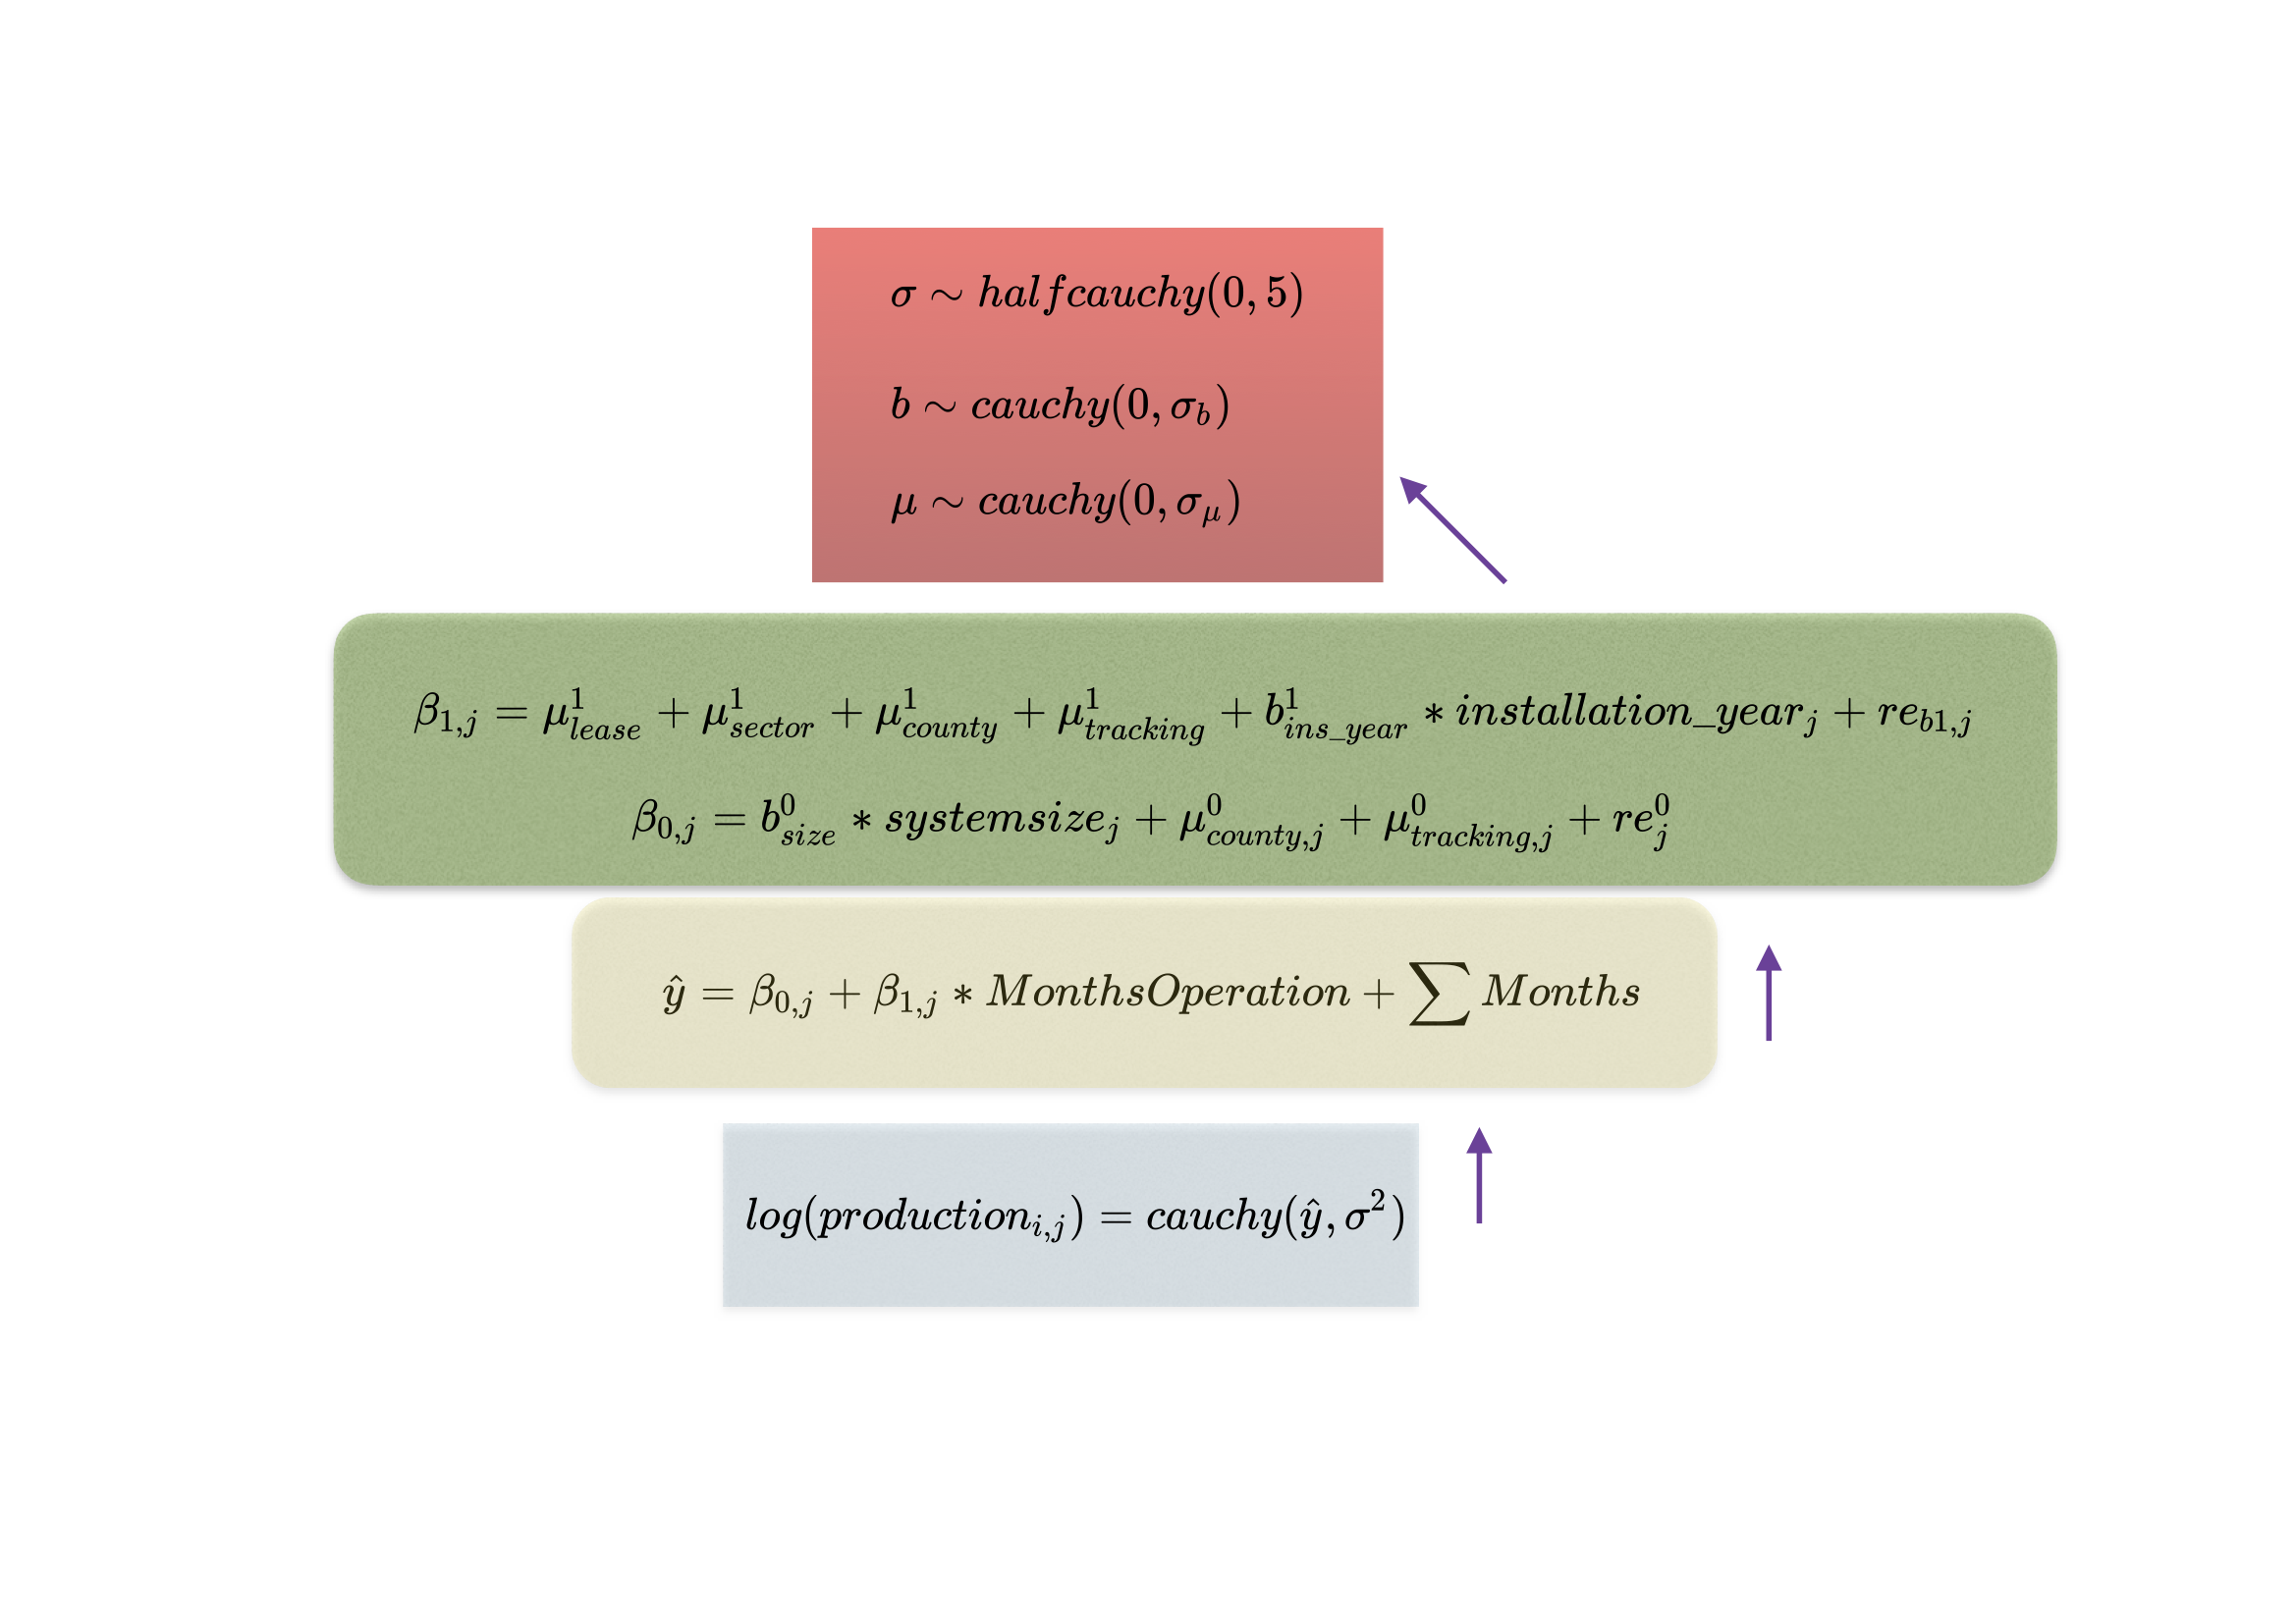
\includegraphics[width=1\textwidth]{figures/solar_prod_bayes_diag.png}
	\caption{The data and the research question combined suggest a hierarchical Bayesian model. The figure shows the structure of the model. Production data is grouped by individual solar panel systems (index i).}
	\label{solar_prod_bayes_diag}
\end{figure}

To estimate the parameters of the model, I use the Stan Bayesian programming language and simulator \citep{stan_development_team_stan_2014} which uses Hamiltonian MCMC to estimate a joint posterior distribution of the parameters. \citet{kruschke_doing_2014} provides an accessible explanation of the Hamiltonian MCMC algorithm, while more detailed technical descriptions are provided by \citet{gelman_bayesian_2013} and \citet{stan_development_team_stan_2014}.

Bayesian simulation methods are still emerging - especially in Economics. So it is worth spending a moment to motivate their use in this case over more common asymptotic methods. As mentioned, the main reason for using the Bayesian model is the flexible treatment it allows for modeling the inherent hierarchy of the data and allowing for partial pooling in estimation.

The usefulness of Bayesian models is most apparent in the estimation of complex hierarchical models with many parameters.
In a hierarchical model, lower-level parameters within a certain group are themselves modeled as coming from a distribution characterized by ``meta-parameters''. Thus, the estimated group-level parameters are a weighted function of both the observations within the group as well as the full set of observations in the dataset. For example, the estimated mean parameter on a group with a few, outlying observations would be pulled towards the full sample mean. This partial pooling also serves as a natural form of parameter shrinkage, which mostly eliminates the need for using corrections for multiple comparisons in inference \citep{gelman_data_2006}.

With Bayesian multilevel model, I also have greater flexibility in specifying the model without having to rely on assumptions like constant group-level variances and a Gaussian noise distribution.  Because Bayesian simulation techniques result in an estimate of the full joint probability distribution of the model, the inference has the potential to be more informative than the typical point estimates and p-values of of the standard hypothesis testing frameworks \citep{kruschke_doing_2014}.

Another advantage is that the posterior distributions of the parameters have a natural and direct interpretation as probabilities, as opposed to standard hypothesis testing where the concepts of p-values and significance are often ill-defined. See \citet{kruschke_doing_2014} or \citet{gelman_bayesian_2013} for further discussion.


\section{Discussion and Conclusion}
The theoretical literature on information asymmetry and quality is established and deep. The empirical literature for consumer durable investments is, however, more sparse, reflecting the difficulty of getting reliable data on purchases and long-term reliability. This article provides one of few case studies that both identifies a market that could be expected to have issues of information asymmetry of quality, and provides an indirect empirical test for the presence of information asymmetry of quality.

The structure of the emerging solar industry in the US, as well as other parts of the world suggests that issues of information asymmetry may play an important role. The established theory on the subject suggests that under information asymmetry of quality, poor quality products may push out good quality products, at least in some sub-markets. In this article I have tested an implication of that theory for the case of solar panels in California. The results provide some weak evidence for the existence of information asymmetry issues of quality.

This article should also be considered as part of a broader literature on the special characteristics of new distributed energy generation technologies. The energy investment behavior of home owners, farmers, and small cooperatives are bound to be substantially different than those of large, specialized energy companies that have traditionally done most of the investment in electricity generation. Understanding the quickly evolving energy and power industry requires taking into account informational and behavioral factors, and this is a rich field for further empirical research

\begin{spacing}{1}
\bibliographystyle{plainnat}
\bibliography{solar_prod}

\FloatBarrier

\appendix
\section{Appendix: Tables}


\end{spacing}
\end{document}
